\documentclass[a4paper,12pt]{article}
\usepackage[utf8]{inputenc}
\usepackage{amsmath}
\usepackage{bm} % to get bold epsilon
\usepackage{amssymb}
\usepackage{comment}
\usepackage{graphicx}
\usepackage{xcolor}
\usepackage[left=1.5cm, right=1.5cm, top=2cm, bottom=2cm]{geometry}
\title{\textbf{COM 5120 Communication Theory}}
\author{\textbf{Practice \#4}}
\date{No need to turn it in, this is for practice purpose only.  \\
Practice and get familiar with the questions are encouraged. \\ 
Some types of the questions might appear on the test. \\}
\begin{document}
    \maketitle
    % \textit{Note: }There are \textbf{6} problems with total 100 points within \textbf{3} pages, please write your answer with detail in the answer sheet.
    % {\bf No credit without detail.  No calculator. Closed books.}
    \begin{enumerate}
    %%%%%%%%%%%%%%%%%%%%%%%%%%%%%%
        \item 
            % 1. (9.38 MLSE)
            Consider the use of a (square-root) raised cosine signal pulse with a roll-off factor of unity for transmission of binary PAM over an ideal band-limited channel that passes the pulse without distortion. Thus, the transmitted signal is 
            \begin{align*}
                v(t) = \sum_{k = -\infty}^{\infty} I_k g_T(t - kT_b)
            \end{align*}
            where the signal interval $T_b = \frac{1}{2}T$. Thus, the symbol rate is double of that for no ISI. \\ 
            (a) Determine the ISI values at the output of a matched filter demodulator. \\
            (b)  Sketch the trellis for the maximum-likelihood sequence detector and label the states. \\ \\
            \textbf{Solution:} \\
            \textbf{(a)} The output of the matched filter demodulator is: 
            \begin{align*}
                y(t) &= \sum_{k = -\infty}^{\infty} I_k \int_{-\infty}^{\infty} g_T(\tau - kT_b)g_R(t - \tau) d\tau + \nu(t) \\ 
                     &= \sum_{k = -\infty}^{\infty} I_k x(t - kT_b) + \nu(t)
            \end{align*}
            where, 
            \begin{align*}
                x(t) = g_T(t) \ \star \ g_R(t) = \frac{\sin \frac{\pi t}{T}}{\frac{\pi t}{T}} \frac{\cos \frac{\pi t}{T}}{1 - 4 \frac{t^2}{T^2}}
            \end{align*}
            Hence, 
            \begin{align*}
                y(mT_b) &= \sum_{k = -\infty}^{\infty} I_k x(mT_b - kT_b) + \nu(mT_b) \\ 
                        &= I_m + \frac{1}{\pi} I_{m - 1} + \frac{1}{\pi} I_{m + 1} + \nu(mT_b)
            \end{align*}
            The term $\frac{1}{\pi} I_{m - 1} + \frac{1}{\pi} I_{m + 1}$ represents the ISI introduced by doubling the symbol rate of transmission. \\
            \newpage
            \textbf{(b)} In Figure 1 we show one trellis stage for the ML sequence detector. Since there is postcursor ISI, we delay the received signal, used by the ML decoder to form the metrics, by one sample. Thus, the states of the trellis correspond to the sequence $\left( I_{m - 1}, I_m \right)$, and the transition labels correspond to the symbol $I_{m + 1}$ . Two branches originate from each state. The upper branch is associated with the transmission of $-1$, whereas the lower branch is associated with the transmission of $1$. 
            \begin{figure}[h]
                \centering
                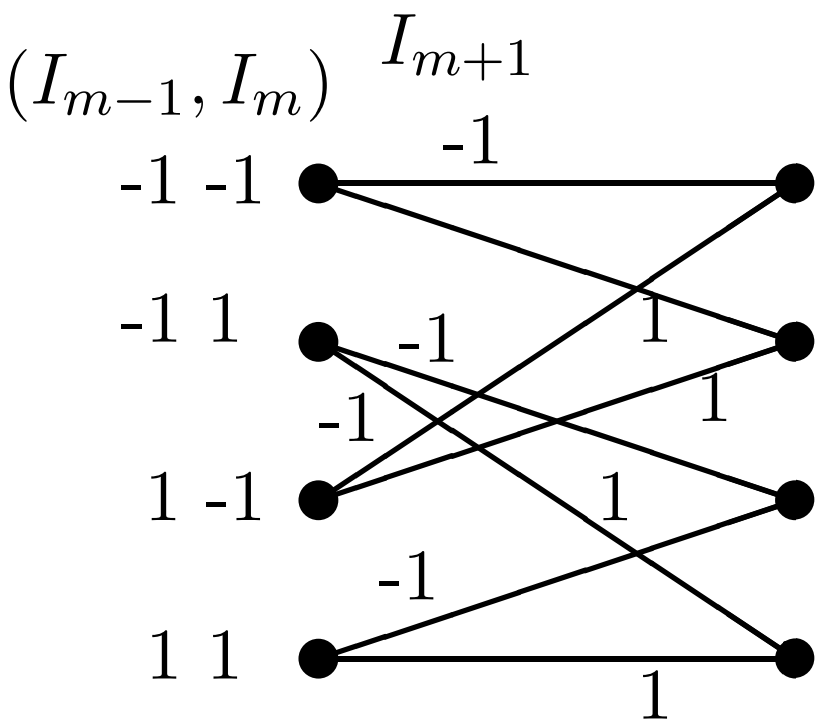
\includegraphics[scale=0.35]{Practice4-1-1.png}
                \caption{trellis stage for the ML sequence detector}
                % \label{fig:my_label}
            \end{figure}
            \begin{flushright}
                $\blacksquare$
            \end{flushright}
    %%%%%%%%%%%%%%%%%%%%%%%%%%%%%%
        \item
            % 2. (9.41 ZF)
            Binary PAM is used to transmit information over an unequalized linear filter channel. When $a = 1$ is transmitted, the noise-free output of the demodulator is
            \begin{align*}
                x_m = \left\{ 
                \begin{aligned}
                    & 0.3 \;\;\;\; m = 1 \\
                    & 0.9 \;\;\;\; m = 0 \\ 
                    & 0.3 \;\;\;\; m = -1 \\
                    & 0 \;\;\;\;\;\; \text{otherwise} \\
                \end{aligned}
            \right.
            \end{align*}
            (a) Design a three-tap zero-forcing linear equalizer so that the output is 
            \begin{align*}
                q_m = \left\{ 
                \begin{aligned}
                    & 1 \;\;\;\; m = 0 \\
                    & 0 \;\;\;\; m = \pm 1 \\ 
                \end{aligned}
                \right.
            \end{align*}
            (b) Determine $q_m$ for $m = \pm 2, \pm 3$, by convolving the impulse response of the equalizer with the channel response. \\ \\ 
            \textbf{Solution:} \\
            \textbf{(a)} The equivalent discrete-time impulse response of the channel is:
            \begin{align*}
                h(t) &= \sum_{n = -1}^{1} h_n \delta(t - nT) \\
                     &= 0.3 \delta(t + T) + 0.9 \delta(t) + 0.3 \delta(t - T)
            \end{align*}
            If by $\{ c_n \}$ we denote the coefficients of the FIR equalizer, then the equalized signal is: 
            \begin{align*}
                q_m = \sum_{n = -1}^{1} c_n h_{m - n}
            \end{align*}
            which in matrix notation is written as: 
            \begin{align*}
                \left(
                \begin{array}{c c c}
                    0.9 & 0.3 & 0.0 \\ 
                    0.3 & 0.9 & 0.3 \\
                    0.0 & 0.3 & 0.9 
                \end{array}
                \right)
                \left(
                \begin{array}{c}
                    c_{-1} \\ 
                    c_0 \\
                    c_1  
                \end{array}
                \right)
                = \left(
                \begin{array}{c}
                    0 \\ 
                    1 \\
                    0  
                \end{array}
                \right)
            \end{align*}
            The coefficients of the zero-force equalizer can be found by solving the previous matrix equation. Thus, 
            \begin{align*}
                \left(
                \begin{array}{c}
                    c_{-1} \\ 
                    c_0 \\
                    c_1  
                \end{array}
                \right)
                =\left(
            \begin{array}{c}
                -0.4762 \\ 
                1.4286 \\
                -0.4762 
            \end{array}
            \right)
            \end{align*}
            \textbf{(b)} The values of $q_m$ for $m = \pm 2, \pm 3$ are given by 
            \begin{align*}
                q_2 &= \sum_{n = -1}^{1} c_n h_{2 - n} = c_1h_1 = -0.1429 \\ 
                q_{-2} &=  \sum_{n = -1}^{1} c_n h_{-2 - n} = c_{-1}h_{-1} = -0.1429 \\
                q_3 &= \sum_{n = -1}^{1} c_n h_{3 - n} = 0 \\ 
                q_{-3} &=  \sum_{n = -1}^{1} c_n h_{-3 - n} = 0
            \end{align*}
            \begin{flushright}
                $\blacksquare$
            \end{flushright}
    %%%%%%%%%%%%%%%%%%%%%%%%%%%%%%
        \item
            % 3. (9.46 MMSE)
            Repeat Problem 2 using the MSE as the criterion for optimizing the tap coefficients. Assume that the noise power spectral density is $0.1$ W/Hz. \\ \\ 
            \textbf{Solution:} \\
            A discrete time transversal filter equivalent to the cascade of the trasmitting filter $g_T(t)$ , the channel $c(t)$, the matched filter at the receiver $g_R(t)$ and the sampler, has tap gain coefficients $\{ x_m \}$, where 
            \begin{align*}
                x_m = \left\{ 
                \begin{aligned}
                    & 0.9 \;\;\;\; m = 0 \\ 
                    & 0.3 \;\;\;\; m = \pm 1 \\
                    & 0 \;\;\;\;\;\; \text{otherwise} \\
                \end{aligned}
            \right.
            \end{align*}
            The noise $\nu_k$, at the output of the sampler, is a zero-mean Gaussian sequence with autocorrelation function:
            \begin{align*}
                E[\nu_k\nu_l] = \sigma^2 x_{k - l}, \;\;\; |k - l| \leq 1
            \end{align*}
            If the $\mathcal{Z}$-transform of the sequence $\{ x_m \}$, $X(z)$, assumes the factorization:
            \begin{align*}
                X(z) = F(z)F^*(z^{-1})
            \end{align*}
            then the filter $1 / F^*(z^{-1})$ can follow the sampler to white the noise sequence $\nu_k$. In this case the output of the whitening filter, and input to the MSE equalizer, is the sequence:
            \begin{align*}
                u_n = \sum_{k} I_k f_{n - k} + n_k
            \end{align*}
            where $n_k$ is zero mean Gaussian with variance $\sigma^2$. The optimum coefficients of the MSE equalizer, $c_k$, satisfy: 
            \begin{align*}
                \sum_{n = -1}^{1} c_n \Gamma_{kn} = \xi_k, \;\;\; k = 0, \pm 1
            \end{align*}
            where: 
            \begin{align*}
                \Gamma(n - k) &= \left\{ 
                \begin{aligned}
                    & x_{n - k} + \sigma^2 \delta_{n, k}, \;\;\;\; |n - k| \leq 1 \\ 
                    & 0 \;\;\;\;\;\;\;\;\;\;\;\;\;\;\;\;\;\;\;\;\;\;\;\; \text{otherwise} \\
                \end{aligned}
                \right.
                \\
                \xi(k) &= \left\{ 
                \begin{aligned}
                    & f_{-k}, \;\;\;\; -1 \leq k \leq 0 \\ 
                    & 0 \;\;\;\;\;\;\;\; \text{otherwise} \\
                \end{aligned}
                \right.
            \end{align*}
            \textcolor{red}{\textbf{[NOTE]}}
            \begin{align*}
                X(z) &= F(z)F^*((\frac{1}{z})^*) = (f_0 + f_1z^{-1})(f_0 + f_1z) \\ 
                     &= f_0^2 + f_1^2 + f_0 f_1z^{-1} + f_0 f_1z = 0.3z + 0.9 + 0.3z^{-1} \\ 
                & \Rightarrow \left\{
                \begin{aligned}
                    & f_0^2 + f_1^2 = 0.9 \\ 
                    & f_0 f_1 = 0.3
                \end{aligned}
                \right. \;\;\;
                \Rightarrow \left\{
                \begin{aligned}
                    & (f_0 + f_1)^2 = 0.9 + 2 \times 0.3 = 1.5 \\ 
                    & f_0 + f_1 = \pm \sqrt{1.5}
                \end{aligned}
                \right. \\ 
                \star \;\; \text{for} \;\; f_0 + f_1 = \; \sqrt{1.5} \;\; \\ 
                f_0 = \frac{0.3}{f_1} & \Rightarrow f_1^2 - \sqrt{1.5}f_1 + 0.3 = 0 \\ 
                                      & \Rightarrow f_1 = \frac{\sqrt{1.5} \pm \sqrt{1.5 - 4 \times 0.3}}{2} = 0.8862 \;\; \text{or} \;\; 0.3385 \\ 
                                      & \;\;\;\;\; f_0 = \frac{0.3}{f_1} = 0.3385 \;\; \text{or} \;\; 0.8862 \\ 
                \star \;\; \text{for} \;\; f_0 + f_1 = -\sqrt{1.5} \\ 
                f_0 = \frac{0.3}{f_1} & \Rightarrow f_1^2 + \sqrt{1.5}f_1 + 0.3 = 0 \\ 
                                      & \Rightarrow f_1 = \frac{-\sqrt{1.5} \pm \sqrt{1.5 - 4 \times 0.3}}{2} = -0.3385 \;\; \text{or} \; -0.8862 \\ 
                                      & \;\;\;\;\; f_0 = \frac{0.3}{f_1} = -0.8862 \;\; \text{or} \; -0.3385
            \end{align*}
            we obtain the parameters $f_0$ and $f_1$ as:
            \begin{align*}
                f_0 = \left\{ 
                \begin{aligned}
                    & \pm \sqrt{0.7854} \; \approx \textcolor{red}{0.8862} \\
                    & \pm \sqrt{0.1146} \; \approx \textcolor{red}{0.3385} \\
                \end{aligned}
                \right. \; \text{, } \;\;\; 
                f_1 = \left\{ 
                \begin{aligned}
                    & \pm \sqrt{0.1146} \; \approx \textcolor{red}{0.3385} \\
                    & \pm \sqrt{0.7854} \; \approx \textcolor{red}{0.8862} \\
                \end{aligned}
                \right.
            \end{align*}
            The parameters $f_0$ and $f_1$ should have the same sign since $f_0f_1 = 0.3$. However, the sign itself does not play any role if the data are differentially encoded. To have a stable inverse system $1 / F^*(z^{-1})$, we select $f_0$ and $f_1$ in such a way that the zero of the system $F^*(z^{-1}) = f_0 + f_1z$ is inside the unit circle. Thus, we choose $f_0 = \sqrt{0.1146} = \textcolor{red}{0.3385}$ and $\textcolor{red}{f_1} = \sqrt{0.7854} = \textcolor{red}{0.8862}$ and therefore, the desired system for the equalizer’s coefficients is
            \begin{align*}
                \left(
                \begin{array}{c c c}
                    0.9 + 0.1 & 0.3 & 0.0 \\ 
                    0.3 & 0.9 + 0.1 & 0.3 \\
                    0.0 & 0.3 & 0.9 + 0.1 
                \end{array}
                \right)
                \left(
                \begin{array}{c}
                    c_{-1} \\ 
                    c_0 \\
                    c_1  
                \end{array}
                \right)
                = \left(
                \begin{array}{c}
                    \sqrt{0.7854} \\ 
                    \sqrt{0.1146} \\
                    0  
                \end{array}
                \right)
                = \left(
                \begin{array}{c}
                    \textcolor{red}{0.8862} \\ 
                    \textcolor{red}{0.3385} \\
                    0  
                \end{array}
                \right)
            \end{align*}
            Solving this system, we obtain 
            \begin{align*}
                c_{-1} = 0.8596, \;\;\; c_{0} =  0.0886, \;\;\; c_{-1} = -0.0266
            \end{align*}
            \begin{flushright}
                $\blacksquare$
            \end{flushright}
    %%%%%%%%%%%%%%%%%%%%%%%%%%%%%%%%%%%%%%%%%%%%%%
    \end{enumerate}
    \rule{\textwidth}{0.4pt}
\end{document}


